Um herauszufinden, welche spezifischen Probleme bestehende CRS im Kontext der Programmierlehre mitbringen, sollen zwei Vertreter miteinander verglichen werden: Einerseits die bisher an der HAW Hamburg eingesetzte Lösung StuReSy und zum Vergleich eine sehr populäre, kommerziellere Lösung namens Pingo.

\section{StuReSy}
\label{chap:sturesy}
\ac{sturesy} ist der Name einer Software, die im Rahmen der Bachelorarbeit von Wolf Posdorfer im Jahr 20012 an der Universität Hamburg entstanden ist. Der Name StuReSy ist ein Akronym für „Student Response System“.

StuReSy besteht aus zwei Komponenten:
\begin{itemize}
    \item Server-Komponente: In PHP geschrieben, agiert gleichzeitig auch als Client-Komponente für die Abstimmungs-Teilenehmer. Inkludiert eine relationale SQL-Datenbank.
    \item Admin-Komponente: Um Fragen zu erstellen und zu bearbeiten wird ein Client als Java-Anwendung benötigt.
\end{itemize}

StuReSy wurde erfolgreich und viele Jahre an der Universität Hamburg und HAW Hamburg eingesetzt. Die Qualität und der Umfang der Software sind für eine Bachelorarbeit beeindruckend.

Dennoch verfügt StuReSy über einige Nachteile und Probleme:
\begin{itemize}
    \item Software-Download und JVM notwendig: Um StuReSy administrativ einsetzen zu können, muss eine Java-Software heruntergeladen werden und eine JVM muss auf dem jeweiligen System vorhanden sein. Eine Administration vom Tablet oder Smartphone ist damit nur schwer möglich.
    \item Server-Komponente: Um StuReSy betreiben zu können, wird eine Server-Instanz benötigt. Diese muss von der jeweiligen Institution oder einem Dozenten aufgesetzt und gewartet werden.
    \item Mangelnde Formatierungsmöglichkeiten für Software-Quelltext: In der Praxis wird StuReSy vor allem in Informatik-Veranstaltungen eingesetzt. Dort werden oft Fragen zu Quelltexten gestellt. Die Darstellung dieser Quelltexte ist schwierig: Zentrierte Text-Ausrichtung .... sorgen für unübersichtliche Darstellung.
\end{itemize}


\newpage
\section{Pingo}
\label{chap:pingo}
Pingo ist eine Software-Lösung, die bereits seit dem Jahr 2011 an der Universität Paderborn entwickelt wird. Der Name ist ebenfalls ein Akronym und steht für „\textbf{P}eer \textbf{In}struction for Very Large \textbf{G}r\textbf{o}ups“. Im Gegensatz zu StuReSy ist Pingo bereits weiter verbreitet und wird an vielen deutschen Hochschulen eingesetzt. Dahinter steht außerdem ein ganzes Team von akademischen Mitarbeitern. Seit 2019 wird Pingo von der universitätsnahen Coactum GmbH betrieben und weiterentwickelt.\newline

Prinzipiell handelt es sich bei Pingo um eine reine Web-Applikation, die öffentlich und kostenlos unter www.trypingo.com zugänglich ist. Für die Nutzung muss jedoch ein Benutzerkonto eröffnet werden. Pingo steht unter einer Open-Source-Lizenz und somit können Nutzer auch eine eigene Pingo-Instanz betreiben. Pingo ist in der Programmiersprache Ruby und mithilfe des Web-Frameworks „Ruby on Rails“ implementiert worden.

Bei den unterstützten Fragetypen sind beide Programme nahezu identisch: Single Choice, Multiple Choice, Freitext und numerische Fragen sind möglich.


Pingo hat prinzipiell einen sehr großen Funktionsumfang, jedoch fehlen entscheidende Funktionen für den Einsatz in der Programmierlehre:
\begin{itemize}
    \item \textbf{Keinerlei Formatierungs-Möglichkeiten}: Fragen innerhalb der Pingo-Plattform können überhaupt nicht formatiert werden. Damit können weder Fettschreibungen, Unterstreichungen oder Zeilenumbrüche verwendet werden. Dementsprechend ist auch die übersichtliche Darstellung von Quelltext vollkommen unmöglich.
\end{itemize}

\begin{figure}[H]
    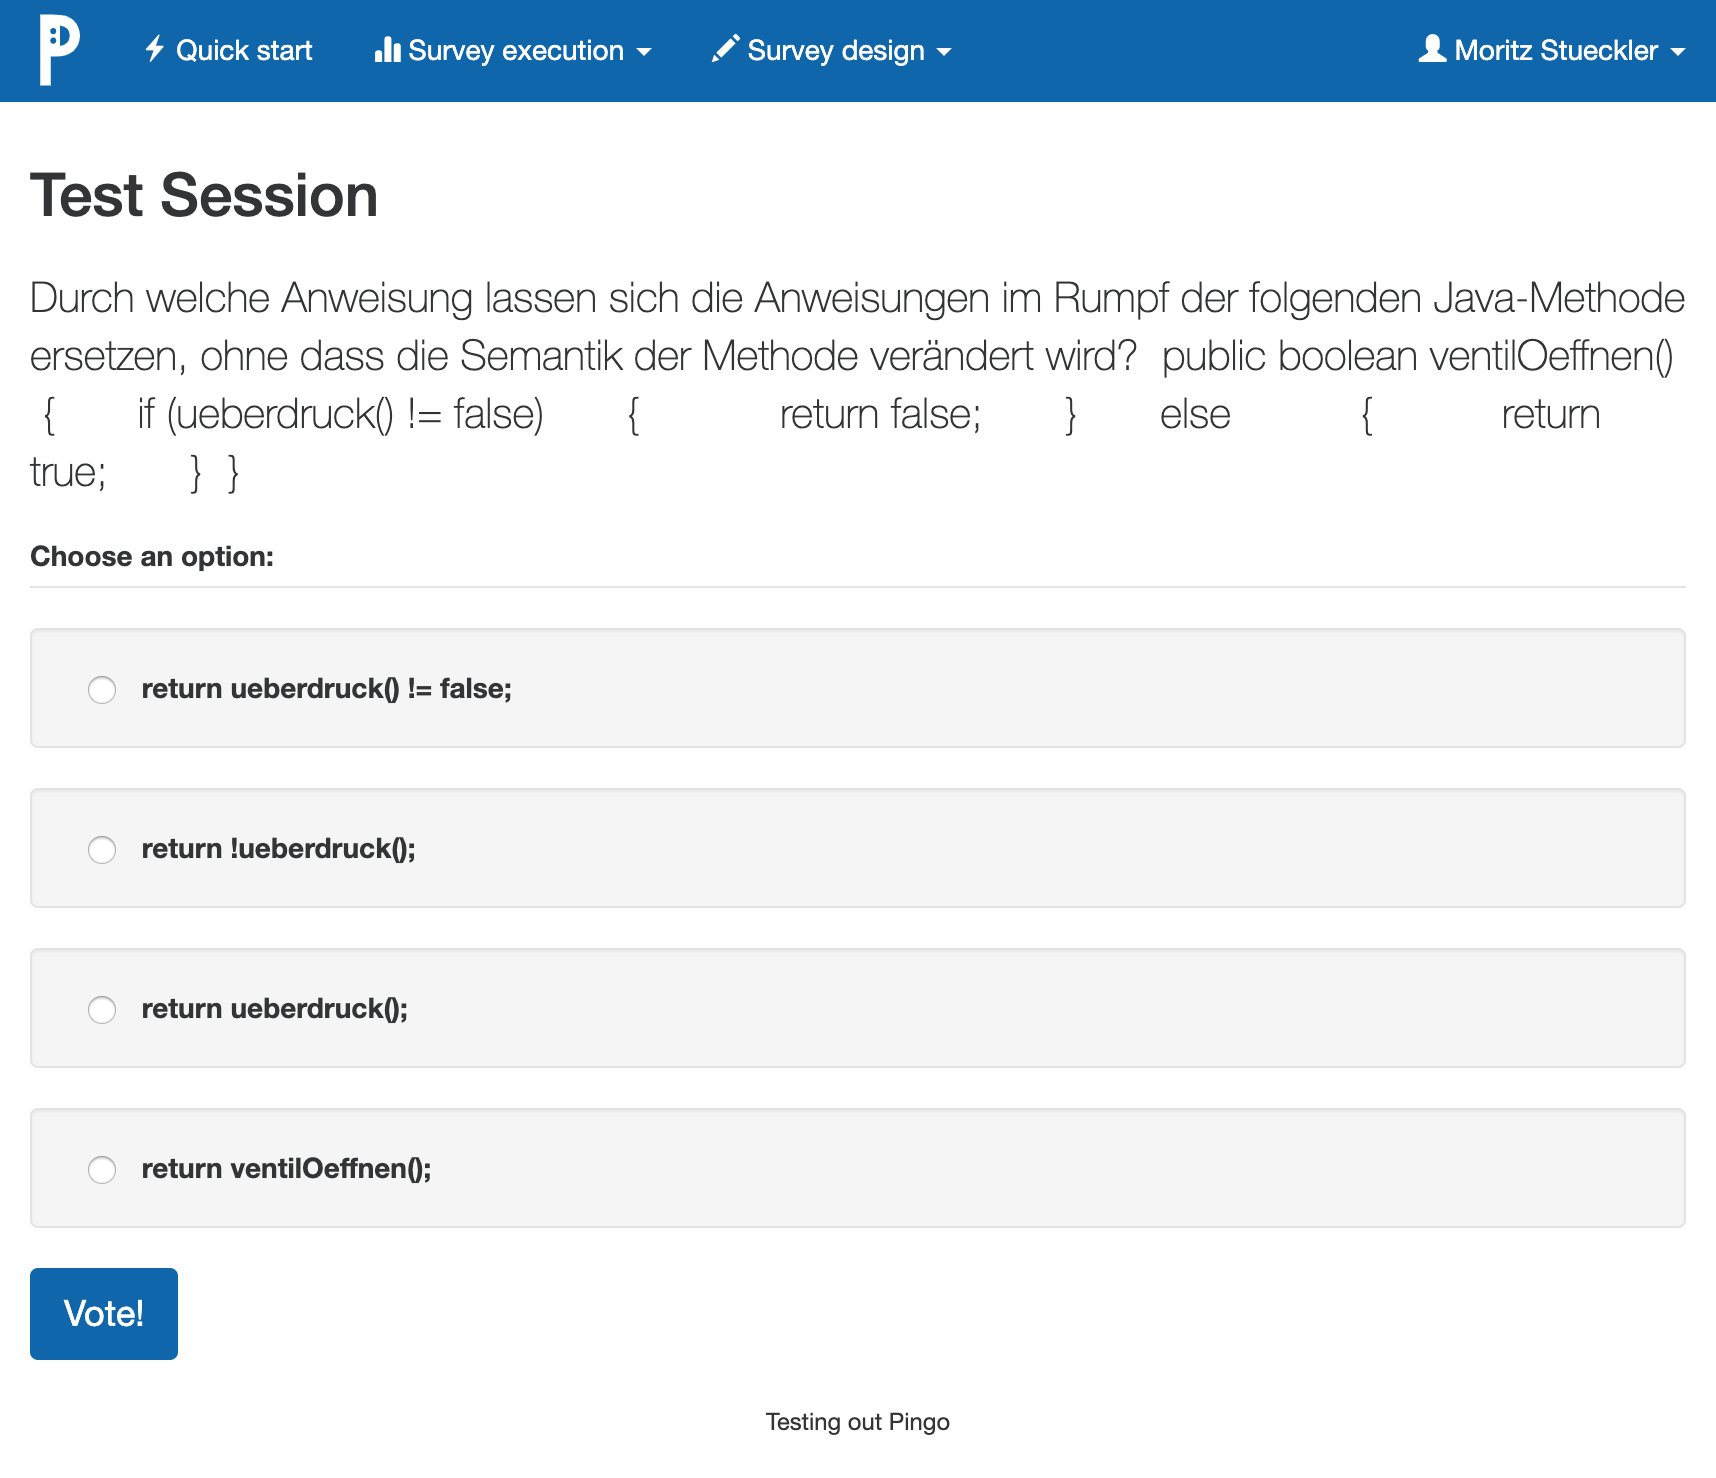
\includegraphics[width=12cm]{chapter/bewertung/bilder/pingo_problem1.png}
    \centering
    \caption{Pingo verfügt über keinerlei Text-Formatierungsoptionen und ist daher ungeeignet für die Darstellung von Quelltext.}
    \label{Abbildung 2.4}
\end{figure}
%
\section{Tabellarische Gegenüberstellung}
\label{chap:tabelle}
 \begin{table}[h]
     \centering
     \caption{Tabellarischer Vergleich verschiedener CRS-Systeme.}
     \label{tab:vergleich}
     \begin{tabular}{|l|c|c|c|}
     \hline
      & \textbf{StuReSy} & \textbf{Pingo} & \textbf{Weclare}  \\
      \hline
      kompl. Webbasiert & x & \checkmark & \checkmark \\
      kommt ohne Server aus & x & x & \checkmark \\
      Code-Formatierungsoptionen & - & x & \checkmark \\
      Code-Ausführung & x & x & \checkmark \\
      \hline
     \end{tabular}
 \end{table}